\documentclass[10pt]{report}

\usepackage{stan-talks}

\begin{document}
\sf%
\mbox{ }
\\[12pt]
\spc{\LARGE\bfseries \color{MidnightBlue}{Taking Uncertainty Seriously}}
\\[4pt]
\spc{\large {for calibrated forecasting and decision making}}
\\[36pt]
\noindent
\spc{\Large\bfseries \color{MidnightBlue}{Bob Carpenter}}
\\[2pt]
\spc{Columbia University}
\vfill
\noindent
\spc{\small October 2019} \hfill
\hfill

\includegraphics[width=0.3in]{img/new-logo.png}

\mypart{}{Motivation}
\pagestyle{plain}

\sld{Scientists}
\pagestyle{plain}
\begin{itemize}
\item want to \myemph{understand} the world,
\item bring mechanistic \myemph{theories},
\item bring data in the form of \myemph{measurements}, and
\item need to make \myemph{predictions} and \myemph{evaluate theories}.
\end{itemize}

\sld{Policymakers}
\begin{itemize}
\item want to \myemph{control} the social world,
\item bring hypotheses about \myemph{interventions},
\item bring data in the form of \myemph{measurements}, and
\item need to \myemph{make decisions} and \myemph{evaluate impact}.
\end{itemize}

\sld{Uncertainty}
\begin{itemize}
\item \myemph{permeates science} and decision making
\item in the form of
\begin{subitemize}
\item \myemph{sampling} uncertainty,
\item \myemph{measurement} uncertainty, and
\item \myemph{modeling} uncertainty.
\end{subitemize}
\vfill
\item The \myemph{alternative to good statistics} is
\begin{subitemize}
\item not no statistics,
\item but \myemph{bad statistics}. \hfill (Bill James)
\end{subitemize}
\end{itemize}

\sld{Probability \& Statistics}
\begin{itemize}
\item Probability theory uses math to \myemph{quantify uncertainty}.
\item \myemph{Bayesian statistics} applies probability theory to
\begin{subitemize}
\item data \myemph{analysis},
\item \myemph{prediction} \& forecasting,
\item model \myemph{evaluation}, and
\item \myemph{decision} theory.
\end{subitemize}
\end{itemize}

\sld{This talk}
\begin{itemize}
\item How to combine data, theory, and probability to
\begin{subitemize}
\item make \myemph{calibrated predictions},
\item \myemph{optimal decisions} under uncertainty, and
\item solve the \myemph{replication crisis}.
\end{subitemize}
\item With \myemph{Stan}, an open probabilistic programming framework
\item Plus a preview of my \myemph{current projects} in
\begin{subitemize}
\item algorithms,
\item methodology and
\item applications.
\end{subitemize}
\end{itemize}

\mypart{}{Calibration}

\sld{Calibration}
\begin{itemize}
\item Empirical (frequentist) evaluation of \myemph{probabilistic forecasts}
\item 75\% of days on which the chance of rain is forecasted at 75\% should be rainy.
\begin{subitemize}
\item for $N$ \myemph{calibrated predictions} of probability $\theta$,
\\
$Y \sim \textrm{binomial}(N, \theta)$ will obtain
\end{subitemize}
\item Depends on \myemph{conditional} information
\item Examples of calibrated predictions of same event
\begin{subitemize}
\item Will it rain in Edinburgh?  (52\%)
\item Will it rain in Edinburgh in December?  (65\%)
\item Will it rain in Edinburgh tomorrow?  (80\%)
\end{subitemize}
\end{itemize}

\sld{Sharpness}
\begin{itemize}
\item Sharp probabilistic predictions are
\begin{subitemize}
\item \myemph{low entropy, high information}
\end{subitemize}
\item \myemph{Narrowly concentrated} predictions are sharper.
\begin{subitemize}
\item $\mbox{Pr}[\alpha \in (.58, .59)] = .9$ sharper than
$\mbox{Pr}[\alpha \in (.5, .6)] = .9$
\end{subitemize}
\item Probabilistic predictions \myemph{nearer 0 or 1} are sharper
\begin{subitemize}
\item $\mbox{Pr}[z_i = 1] = 0.95$ sharper than $\mbox{Pr}[z_i = 1] = 0.6$
\end{subitemize}
\end{itemize}

\sld{Model evaluation criterion}
\begin{itemize}
\item For probabilistic forecasts,
\\
\myemph{maximize sharpness subject to calibration.}
\\[-6pt]
\item \myemph{Goal}: consistent, useful inference from \myemph{finite data}.
\begin{subitemize}
\item cf. minimize variance subject to zero bias for estimators
\end{subitemize}
\item Bayesian models are calibrated if they are \myemph{well-specified}
\begin{subitemize}
\item But, models are always approximate,
\item so need to test with real data.
\end{subitemize}
\end{itemize}

\mypart{}{Demand}

\sld{Pent-up demand for inference}
\vspace*{-3pt}
\begin{itemize}
\item \myemph{Big data} needs \myemph{big model}
\begin{subitemize}
\item temporal structure, spatial structure, missing data, varying effects by group, non-linearity, correlated effects, meta-analysis, heterogeneous data, biased samples, $\ldots$
\item adjust from sample to population, from control to treatment groups, and
from measurements to latent variables
\item this all requires modeling
\end{subitemize}
\item Data size \& computation limit practical model complexity
\item \myemph{Goal}: push the efficient frontier (already pushed $10^2{-}\infty$)
\begin{center}
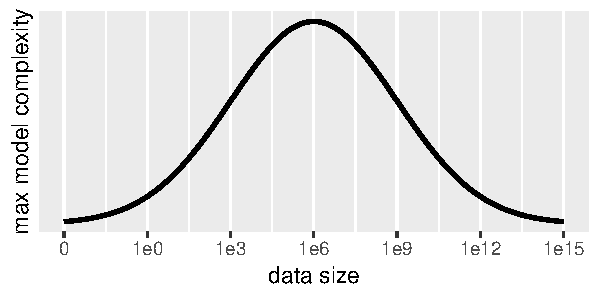
\includegraphics[width=0.5\textwidth]{img/model-size.pdf}
\end{center}
\end{itemize}



\mypart{}{Bayesian Inference}

\sld{Notation}
\begin{itemize}
\item Variables
\begin{subitemize}
\item $y$ : \myemph{data} (observed)
\item $\theta$ : \myemph{parameters} (unknown)
\end{subitemize}
\item Probability functions
\begin{subitemize}
\item $p(y, \theta)$ : \myemph{joint} density
\item $p(y \mid \theta)$ : \myemph{sampling} density
{\footnotesize \hfill (\myemph{likelihood} as fun of $\theta$)}
\item $p(\theta)$ : \myemph{prior} (parameter marginal)
\item $p(\theta \mid y)$ : \myemph{posterior}
\item $p(y)$ : \myemph{evidence} (data marginal)
\end{subitemize}
\end{itemize}

\sld{Bayes's rule}
{\footnotesize
\begin{eqnarray*}
p(\theta \mid y) & = & \frac{p(y, \theta)}{p(y)}
\\[4pt]
& = & \frac{p(y \mid \theta) \cdot p(\theta)}{p(y)}
\\[4pt]
& = & \frac{p(y \mid \theta) \cdot p(\theta)}{\int_{\Theta} p(y, \theta) \, \textrm{d}\theta}
\\[4pt]
& = & \frac{p(y \mid \theta) \cdot p(\theta)}{\int_{\Theta} p(y \mid \theta) \cdot p(\theta) \, \textrm{d}\theta}
\\[10pt]
& \propto &
p(y \mid \theta) \cdot p(\theta).
\end{eqnarray*}
\begin{subitemize}
\item \myemph{Posterior} proportional to \myemph{likelihood times prior}
\end{subitemize}
}

\sld{Estimates, events, and predictions}
\begin{itemize}
\item \myemph{Parameter estimate}
$$
\hat{\theta}
\ = \ \mathbb{E}\!\left[\theta \mid y\right]
\ = \
\int_{\Theta} \theta \cdot p(\theta \mid y) \, \textrm{d}\theta
$$
\item \myemph{Event probability} ($A \subseteq \Theta$, \ \ {\footnotesize e.g., $A = \{ \theta : \theta > 0\}$})
$$
\textrm{Pr}[A \mid y]
\ = \ \mathbb{E}\!\left[\textrm{I}_A(\theta) \mid y\right]
\ = \
\int_{\Theta} \textrm{I}_A(\theta) \cdot p(\theta \mid y)
\, \textrm{d}\theta
$$
\item \myemph{Predictive inference}
$$
p(\tilde{y} \mid y)
\ = \ \mathbb{E}\!\left[p(\tilde{y} \mid \theta) \ \middle| \ y\right]
\ = \
\int_{\Theta} p(\tilde{y} \mid \theta) \cdot p(\theta \mid y)
\, \textrm{d} \theta
$$
\end{itemize}

\sld{(Markov chain) Monte Carlo}
\begin{subitemize}
\item Given \myemph{sample} $\theta^{(1)}, \ldots, \theta^{(M)} \sim p(\theta \mid y).$
\item General \myemph{plug-in expectation} calculations,
\begin{eqnarray*}
\mathbb{E}[f(\theta) \mid y]
& = &
\int_{\Theta} \, f(\theta) \cdot p(\theta \mid y) \, \textrm{d}\theta
\\[8pt]
& = &
\lim_{M \rightarrow \infty} \,
\frac{1}{M} \, \sum_{m=1}^M \, f\!\left(\theta^{(m)}\right)
\\[8pt]
& \approx &
\frac{1}{M} \, \sum_{m=1}^M \, f\!\left(\theta^{(m)}\right).
\end{eqnarray*}
\item (MCMC) central limit theorem \myemph{approx. error} $\mbox{ } \propto \frac{\displaystyle 1}{\displaystyle \sqrt{M}}$
\end{subitemize}

\mypart{Decision Theory}

\sld{Expected utility and risk}
\begin{itemize}
\item Agent has choice of \myemph{actions} $a \in A$.
\begin{subitemize}
\item discrete: do I go to college?
\item continuous: how much do I invest for retirement?
\end{subitemize}
\item \myemph{Utility}: $\textrm{util}(a, \theta)$ based on state of world $\theta$
\begin{subitemize}
\item risk aversion, etc. rolled into utility
\end{subitemize}
\item \myemph{Expected Utility} conditioned on $y$:
$$
\mathbb{E}\!\left[\textrm{util}(a, \theta) \mid y\right]
\ = \
\int_{\Theta} \textrm{util}(a, \theta) \cdot p(\theta \mid y) \ \textrm{d}\theta.
$$
\item point estimates aren't plug \& play due to \myemph{non-linearity}
\end{itemize}

\sld{Optimal Decisions}
\begin{itemize}
\item Given observed data $y$ and model $p(y, \theta)$, choose action $a^* \in A$ that \myemph{maximizes expected utility}
$$
a^* = \textrm{arg max}_\theta \ \mathbb{E}\!\left[\textrm{util}(a, \theta) \mid y\right].
$$
\item \myemph{Compute} expectation via MCMC sample
$$
\theta^{(1)}, \ldots, \theta^{(m)} \sim p(\theta \mid y),
$$
as
$$
\mathbb{E}\!\left[\textrm{util}(a, \theta) \mid y\right]
\ \approx \
\frac{1}{M} \sum_{m=1}^M \textrm{util}(a, \theta^{(m)})
$$
\item This objective can be \myemph{automatically differentiated}.
\end{itemize}

\sld{Online A/B/... testing}
\begin{itemize}
\item Discrete sequence of actions $a_1, \ldots, a_T \in 1:K$
\item Model of actions $p(y \mid \theta_k)$
\item and utility $\textrm{util}(\theta, a)$
\item choose next action with probability proportional to expected utility.
\begin{subitemize}
\item known as Thompson sampling in the bandit literature
\end{subitemize}
\vfill {\footnotesize Student project with Dinko Franceschi, Andrew Gelman, and Lauren Kennedy}
\end{itemize}

\mypart{Bayesian Workflow}

\sld{Bayesian Workflow}
\begin{enumerate}
\item design experiment \& collect data (big workflow here)
\item for gradually \myemph{increasing model complexity}
\begin{subitemize}
\item \myemph{test model} and sofware on simulated data,
\item \myemph{fit model} to real data,
\item perform posterior predictive checks (\myemph{does it fit data?}),
\item perform held-out checks or cross-validation (\myemph{does it predict?}).
\end{subitemize}
\vfill
{\footnotesize Simpson, Rajagopal, Morris, Kennedy, Gelman, Carpenter.  (forthcoming) {\it Bayesian Workflow in Stan}. CRC Press. \url{https://github.com/jgabry/bayes-workflow-book}}
\end{enumerate}

\mypart{Example 1}{Birth Ratio}

\sld{Birth ratio \hfill {\Large (Laplace, 1781)}}
\begin{itemize}
\item \myemph{Live births} in Paris, 1745--1770
\begin{subitemize}
\item $y = 251,527$ male, $N = 493,472$ total
\end{subitemize}
\item \myemph{Sampling}:
$p(y \mid N, \theta)
 = \textrm{binomial}(y \mid N, \theta).$
\item \myemph{Prior}:
$p(\theta)
 = \textrm{uniform}(\theta \mid 0, 1)$
\item \myemph{Posterior}:
$p(\theta \mid y)
 = \textrm{beta}(\theta \mid 1 + y, \ 1 + N - y).$
\vfill
\item {$\textrm{Pr}[\theta \in (0.508, 0.512)] = 0.99$}
\hfill {\small (estimated \myemph{male birth rate})}
\item {$\textrm{Pr}[\theta > 0.5] \approx 1 - 10^{-42}$}
\hfill {\small (``morally certain'' \myemph{more boys})}
\end{itemize}

\sld{Coding in Stan}
\begin{stancode}
transformed data {
  int y = 251527;  int N = 493472;
}
parameters {
  real<lower=0, upper=1> theta;
}
model {
  y ~ binomial(N, theta);
}
generated quantities {
  int<lower=0, upper=1> theta_gt_half = (theta > 0.5);
  int<lower = 0> y_sim = binomial_rng(100, theta);
}
\end{stancode}

\sld{Executing}
%
\begin{codein}
> fit <- stan("laplace.stan")
> print(fit, probs=c(0.005, 0.995), digits=3)
\end{codein}
\begin{codeout}
                     mean se_mean   0.5%   99.5%
theta               0.510   0.000  0.508   0.512
theta_gt_half       1.000     NaN  1.000   1.000
y_sim              50.902   0.081 38.000  64.000
\end{codeout}
%
\begin{subitemize}
\item \myemph{estimate} $\hat{\theta}$ is posterior sample \myemph{mean} for $\theta$;
\item 99\% \myemph{interval} for $\theta$ estimated by sample \myemph{quantiles}
\item $\textrm{Pr}[\theta > 0.5]$ estimated by sample \myemph{mean of indicator}
\item {\texttt y\_sim} estimated \myemph{forecast} for next 100 births
\end{subitemize}


\mypart{Example 2}{Population Dynamics}

\sld{Population Dynamics \hfill {\large (Volterra 1926)}}
\begin{itemize}
\item populations at $t$ of prey $u(t)$ \& predator $v(t)$
\item Volterra's mechanistic model
$$
\frac{\textrm{d}}{\textrm{d}t}u = (\alpha - \beta \cdot v) \cdot u
\qquad
\frac{\textrm{d}}{\textrm{d}t}v = (-\gamma + \delta \cdot u) \cdot v
$$
\vspace*{-12pt}
\begin{subitemize}
\item $\alpha$: prey growth rate;  \ $\beta$: predation shrinkage
\item $\gamma$: predator shrinkage; \ $\delta$: predation growth
\end{subitemize}
\end{itemize}

\sld{Analytic solution \hfill {\large (Volterra 1926)}}
\begin{center}
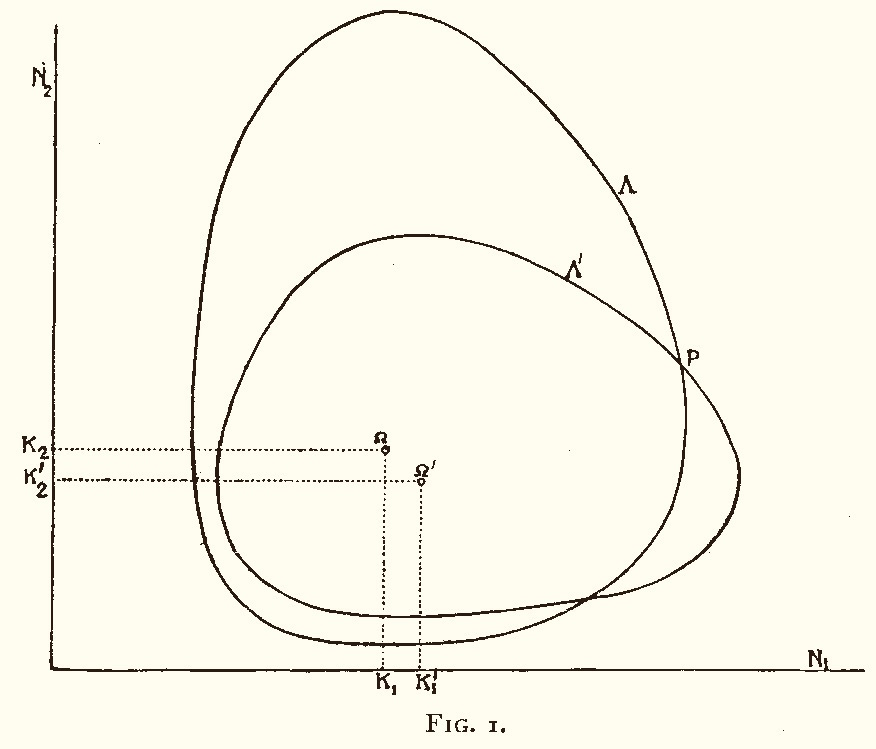
\includegraphics[width=0.6\textwidth]{img/volterra-solutions.jpg}
\end{center}

\sld{Measurement error}
\begin{itemize}
\item $u, v$ are observed
\item $\hat{u}, \hat{v}$ predicted by mechanistic model
\item Independent error proportional to population size
\begin{subitemize}
\item $u_t \sim \textrm{lognormal}(\hat{u}_t, \sigma_1)$
\item $v_t \sim \textrm{lognormal}(\hat{v}_t, \sigma_2)$
\end{subitemize}
\item Weakly informative priors inform scale
\begin{subitemize}
\item $\alpha, \gamma \sim \textrm{normal}(1, 0.5)$; \ \ \
$\beta, \delta \sim \textrm{normal}(0.05, 0.05)$
\item $\sigma_1, \sigma_2 \sim \textrm{lognormal}(-1, 1)$
\end{subitemize}
\end{itemize}

\sld{Hudson's Bay Co.\ pelts \hfill {\large (Hewitt 1921)}}
\begin{center}
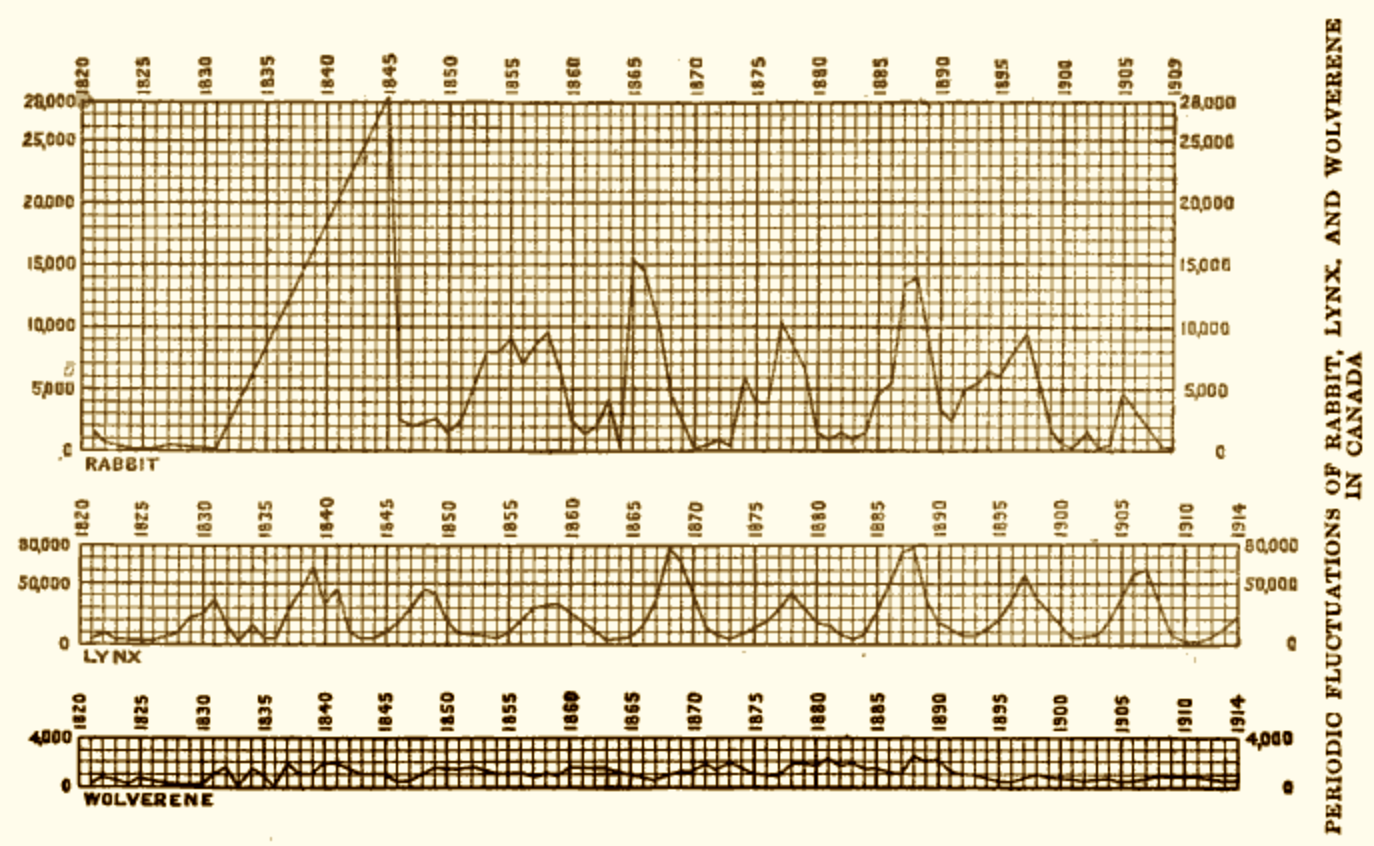
\includegraphics[width=0.9\textwidth]{img/hudons-bay-data.png}
\end{center}

\sld{Plotted pelt data}
\begin{center}
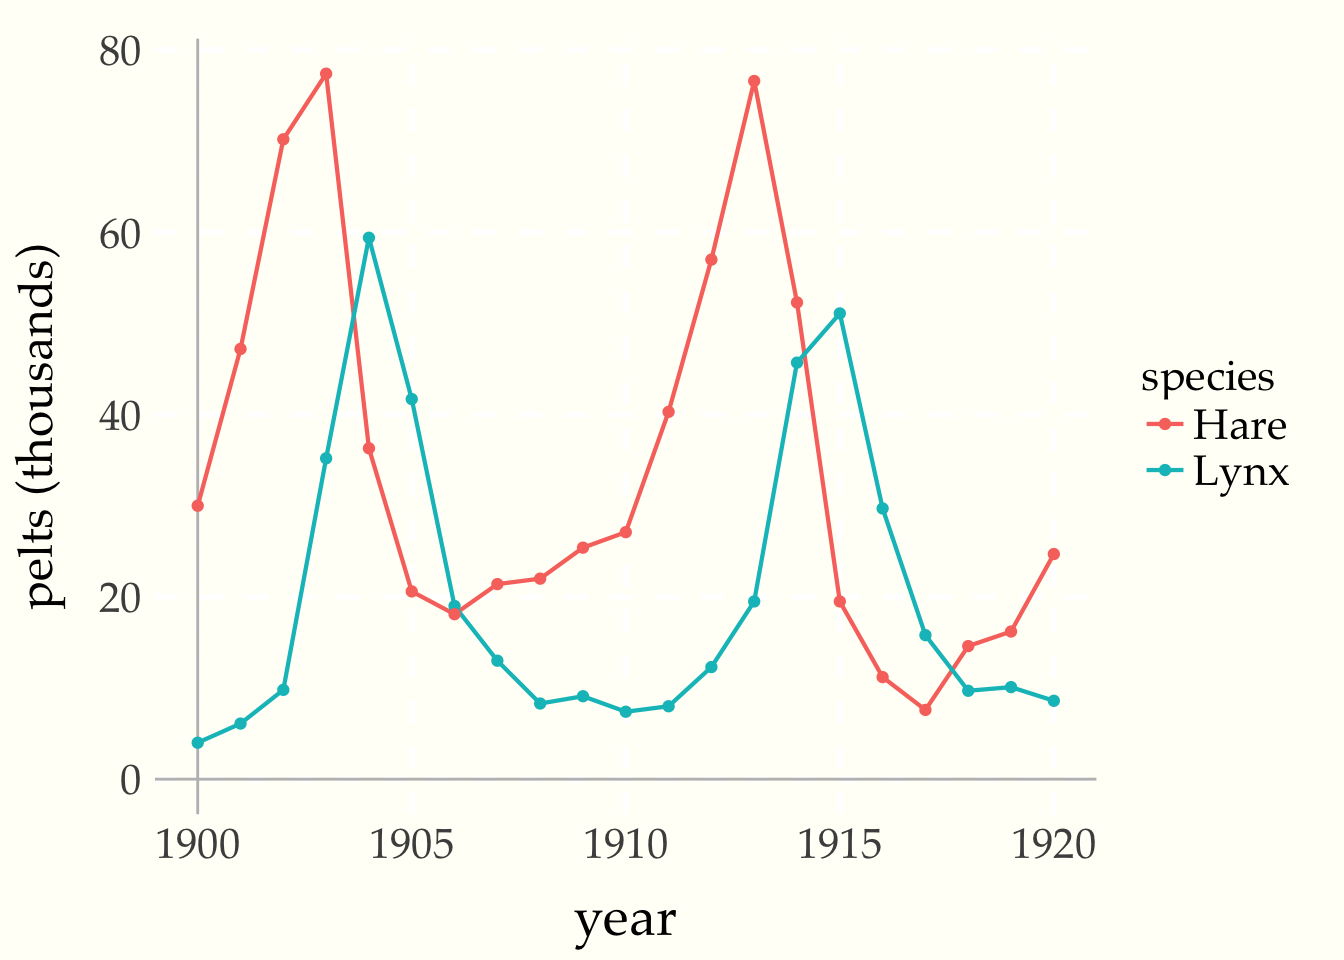
\includegraphics[width=0.45\textwidth]{img/lynx-hares-1.png}~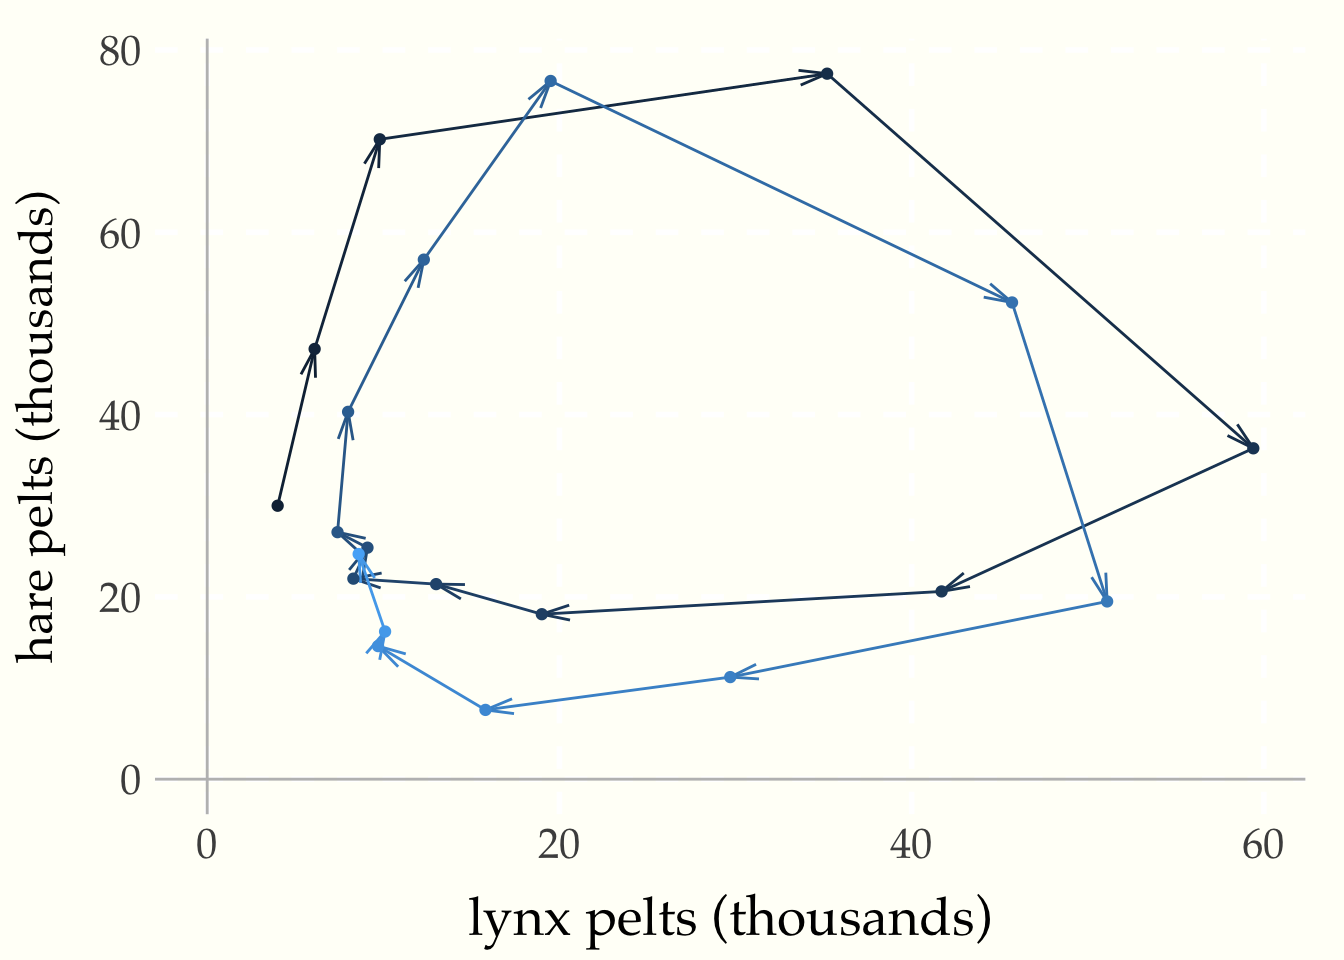
\includegraphics[width=0.45\textwidth]{img/lynx-hares-2.png}
\end{center}
\begin{itemize}
\item {\it left)} pelts vs. time \hfill
{\it right)} hare vs. lynx pelts
\\
(line per species) \hfill (over time)
\end{itemize}

\sld{Stan dynamics \& error}
\begin{stancode}
real[] dz_dt(real t, real[] uv, real[] theta,
             real[] theta, real[] x_r, int[] x_i) {
  return { (theta[1] - theta[2] * uv[2]) * uv[1],
           (-theta[3] + theta[4] * uv[1]) * uv[2] };
}
...
real z[T, 2]
  = integrate_ode(dz_dt, z0, t0, sol_ts[1:T], theta,
                  rep_array(0.0, 0), rep_array(0, 0));
...
y[1:T, 1] ~ lognormal(z[1:T, 1], sigma_u);
y[1:T, 2] ~ lognormal(z[1:T, 2], sigma_v);
\end{stancode}

\sld{Measurements \& predictions}
\begin{center}
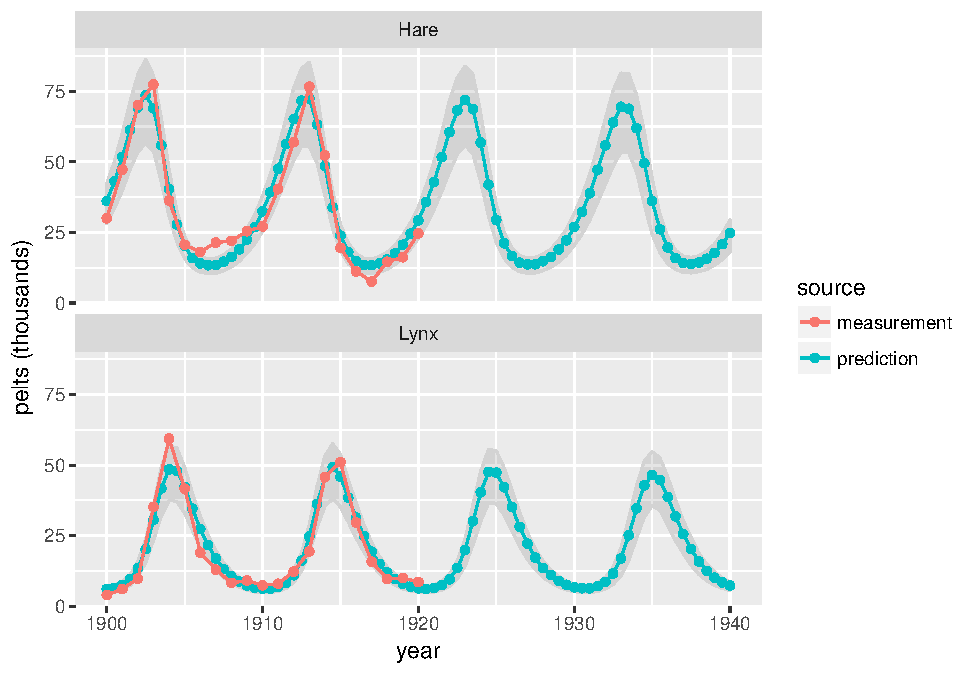
\includegraphics[width=0.8\textwidth]{img/lotka-volterra-posterior.pdf}
\end{center}

\sld{100 predictive draws}
\begin{center}
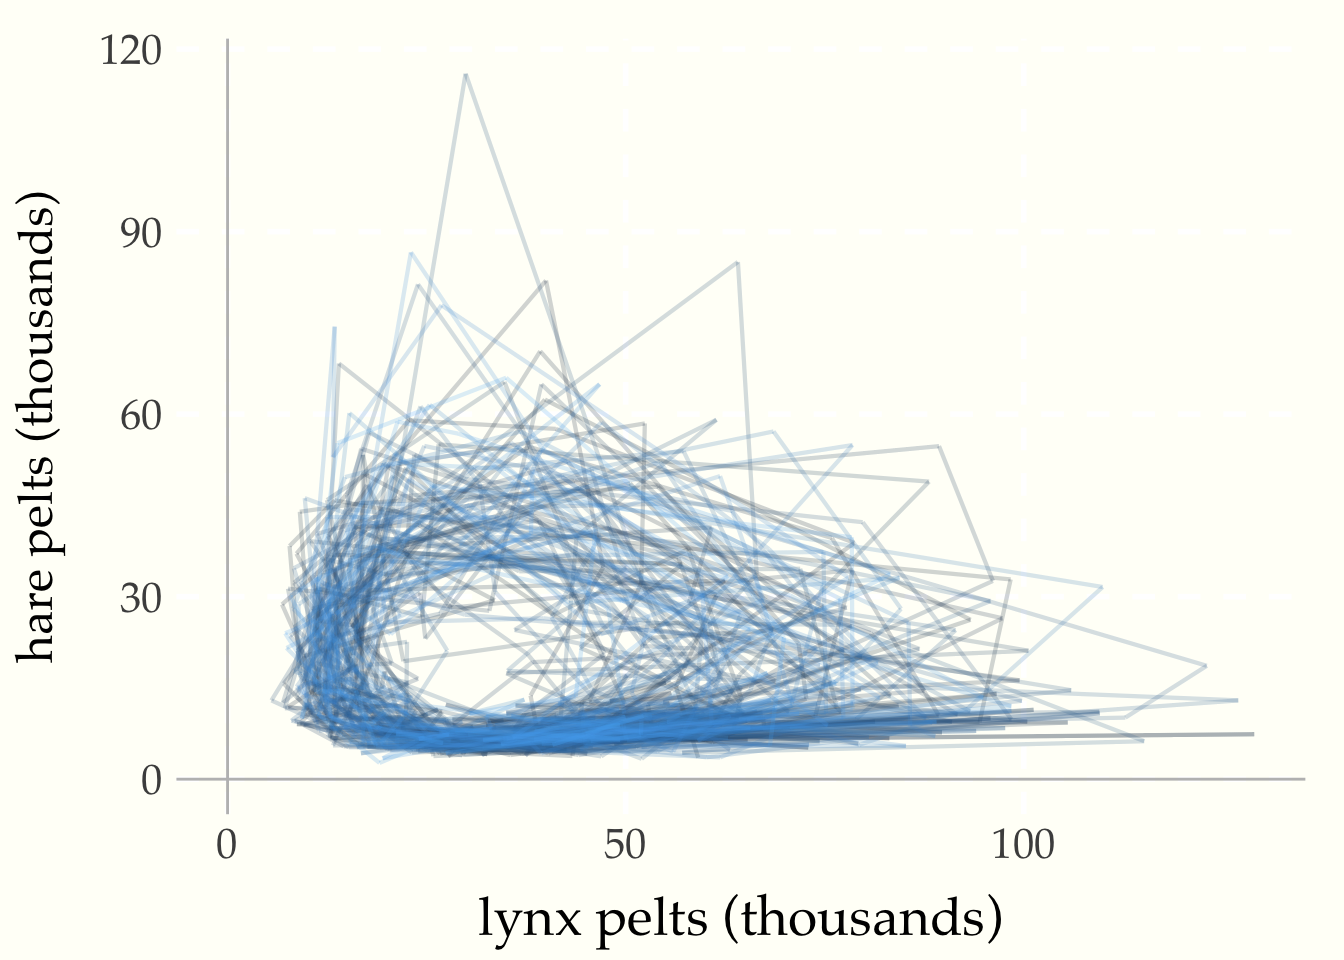
\includegraphics[width=0.8\textwidth]{img/lotka-volterra-posterior-time.png}
\end{center}

\sld{Summary}
\begin{itemize}
\item mechanistic forward model of dyamics (Lotka 1926) $\hat{y} = f(\theta)$
\item noisy measurement model $y_{t,k} \sim \textrm{lognormal}(\hat{y}_{t,k}, \sigma_k)$
\item added weakly informative priors (roughly fixing scale) $p(\theta)$
\item turn the Bayesian crank to sample from posterior
\begin{subitemize}
\item $\theta^{(1)}, \ldots, \theta^{(M)} \sim p(\theta \mid y).$
\end{subitemize}
\item This methodology \myemph{works for many scientific models}.
\end{itemize}

\mypart{Example 3}{Linear Models}

\sld{Logistic regression}
%
\begin{stancode}
 data {
   int<lower = 1> K;
   int<lower = 0> N;
   matrix[N, K] x;                  // predictors
   int<lower=0, upper=1> y[N];      // observations
 }
 parameters {
   vector[K] beta;                  // regression coeffs
 }
 model {
   beta ~ normal(0, 2);            // prior
   y ~ bernoulli_logit(x * beta);  // likelihood
 }
\end{stancode}

\sld{Linear regression with prediction}
%
\begin{stancode}
data {
  int<lower=0> K;
  int<lower=0> N;           int<lower=0> N_tilde;
  matrix[N, K] x;           matrix[N_tilde, K] x_tilde;
  vector[N] y;
}
parameters {
  vector[K] beta;           real<lower=0> sigma;
}
model {
  y ~ normal(x * beta, sigma);
}
generated quantities {
  vector[N_tilde] y_tilde
    = normal_rng(x_tilde * beta, sigma);
}
\end{stancode}

\sld{Time series autoregressive: AR(1)}
%
\begin{stancode}
  data {
    int<lower=0> N;   vector[N] y;
  }
  parameters {
    real alpha;  real beta;  real sigma;
  }
  model {
    y[2:n] ~ normal(alpha + beta * y[1:(n-1)], sigma);
  }
\end{stancode}

\sld{Priors with covariance}
%
\vspace*{-3pt}
\begin{subitemize}
\item $G$ groups w.\ varying slope and intercept; \code{gg[n]} indicates group
\vspace*{-4pt}
\item LKJ prior concentrates around unit correlation
 (${ } \propto \textrm{det}(\Omega)^{\eta - 1}$)
\vspace*{-4pt}
\item Cholesky-factor parameterization for efficiency ($\Omega = \textrm{L}_{\Omega} \cdot \textrm{L}_{\Omega}^{\top}$)
\end{subitemize}
\vspace*{-8pt}
\begin{stancode}
parameters {
  vector[2] beta[G];
  cholesky_factor_corr[2] L_Omega;
  vector<lower = 0>[2] sigma;

model {
  matrix[2, 2] L_Sigma = diag_pre_multiply(sigma, L_Omega);
  sigma ~ normal(0, 2);
  L_Omega ~ lkj_cholesky(4);
  beta ~ multi_normal_cholesky(zeros(2), L_Sigma);

  y ~ bernoulli_logit(... + x .* beta[gg]);
\end{stancode}

\sld{Gaussian process}
%
\vspace*{-5pt}
\begin{stancode}
data {
  int<lower=1> N;  vector[N] x; vector[N] y;
} parameters {
  real<lower=0> eta_sq, inv_rho_sq, sigma_sq;
} transformed parameters {
  real<lower=0> rho_sq; rho_sq = inv(inv_rho_sq);
} model {
  matrix[N,N] Sigma;
  for (i in 1:(N-1)) {
    for (j in (i+1):N) {
      Sigma[i,j] = eta_sq * exp(-rho_sq * square(x[i] - x[j]));
      Sigma[j,i] = Sigma[i,j];
  }}
  for (k in 1:N) Sigma[k,k] = eta_sq + sigma_sq;
  eta_sq, inv_rho_sq, sigma_sq ~ cauchy(0,5);
  y ~ multi_normal(rep_vector(0,N), Sigma);
}
\end{stancode}

\mypart{Example 4}
       {Gene Splice Variants}

\sld{Project}
\begin{itemize}
\item \myemph{Joint work} with
\begin{subitemize}
\item \myemph{Shuonan Chen} (Columbia Uni., biostats)
\item Chaolin Zhang (Columbia Uni., genomics)
\end{subitemize}
\item \myemph{Hierarchical model} with \myemph{full Bayes} follows biology
\item Dramatically \myemph{outperforms} the \myemph{state of the art}:
\begin{quote}
\footnotesize Shihao Shen et al. 2014. rMATS: Robust and flexible detection of
differential alternative splicing from replicate RNA-Seq data.
{\slshape PNAS}.
\end{quote}
\item Simulation tests generated as in Shen et al.
\item No magic---we just \myemph{turned the Bayesian crank} using Stan.
\end{itemize}

\sld{Cassette exons}
\begin{center}
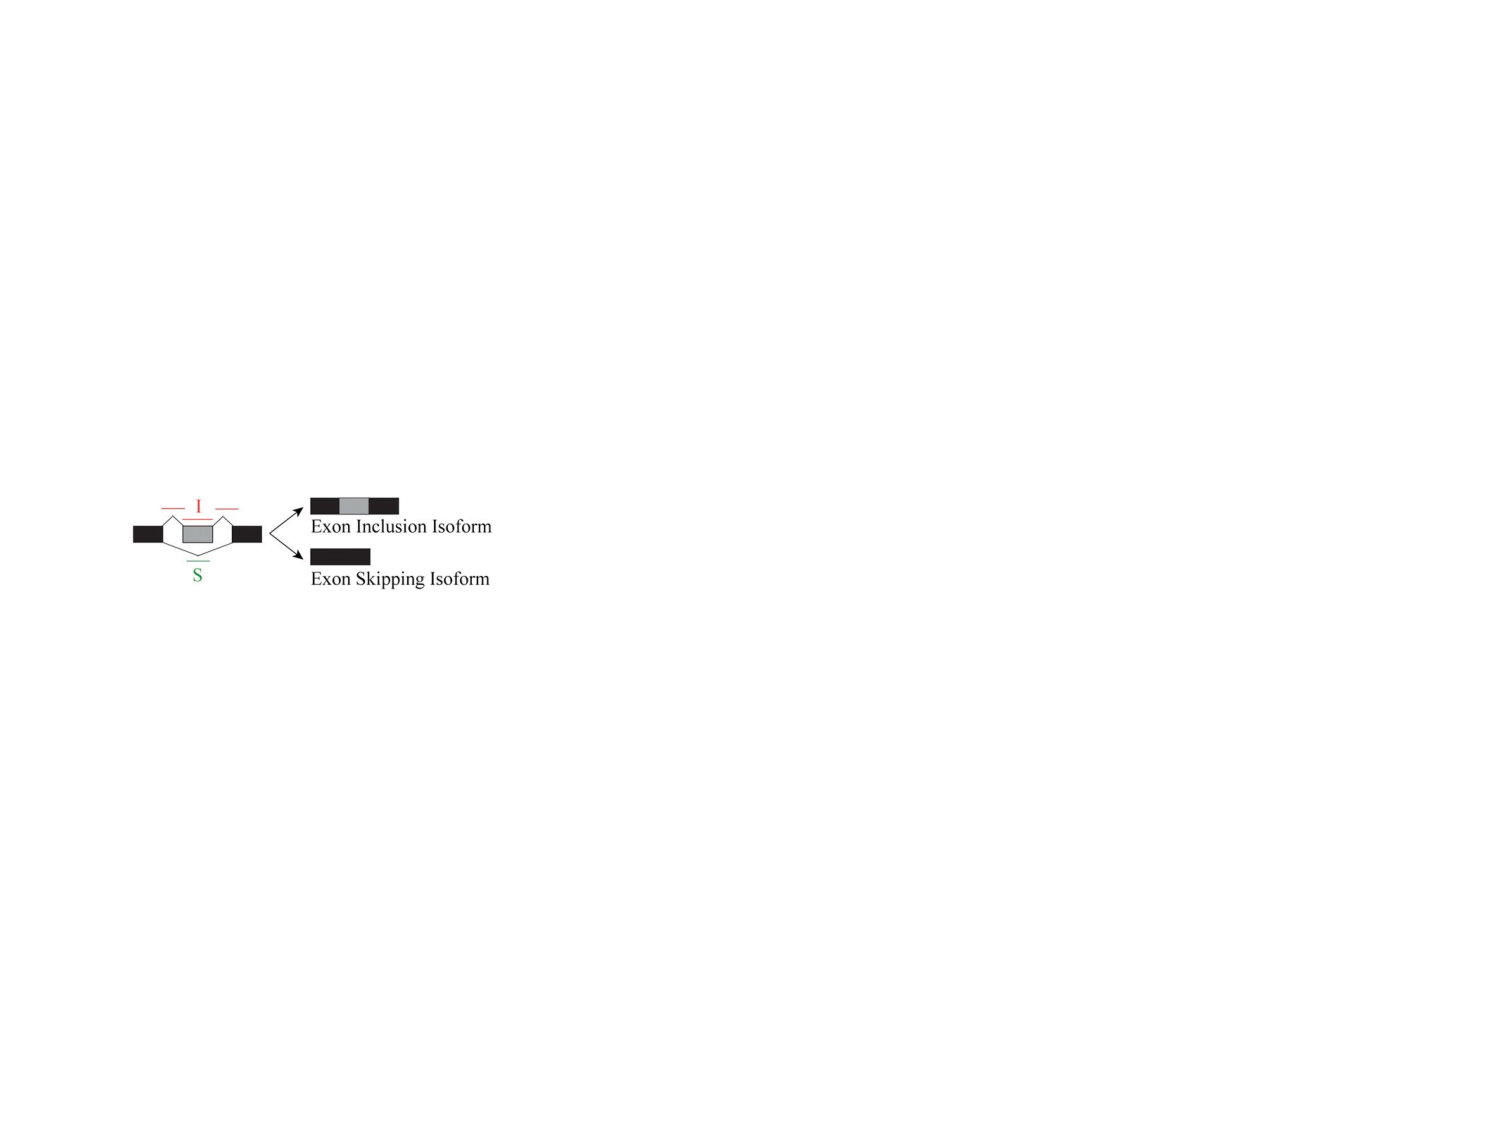
\includegraphics[width=0.8\textwidth]{img/cassette-exon.pdf}
\end{center}
\begin{itemize}
\item Genes are sequences of exons and introns.
\item During transcription, introns skipped and \myemph{exons spliced}.
\item Skipping \myemph{cassette exons} translates \myemph{different proteins}.
\item Different \myemph{cell types} have different proportions of isoforms.
\item There is further \myemph{individual variation}.
\end{itemize}

\sld{RNA sequencing data}
\begin{itemize}
\item Isoforms (seqs. of exons) \myemph{translated} from DNA to RNA.
\item Isoform \myemph{expression} varies by type, condition, and subject.
\item RNA-seq tech.\ \myemph{samples and sequences} RNA inexpensively.
\item Alignment software \myemph{maps} RNA seqs.\ to \myemph{genome position}.
\item Raw data is \myemph{alignment counts}:
\end{itemize}
\begin{center}
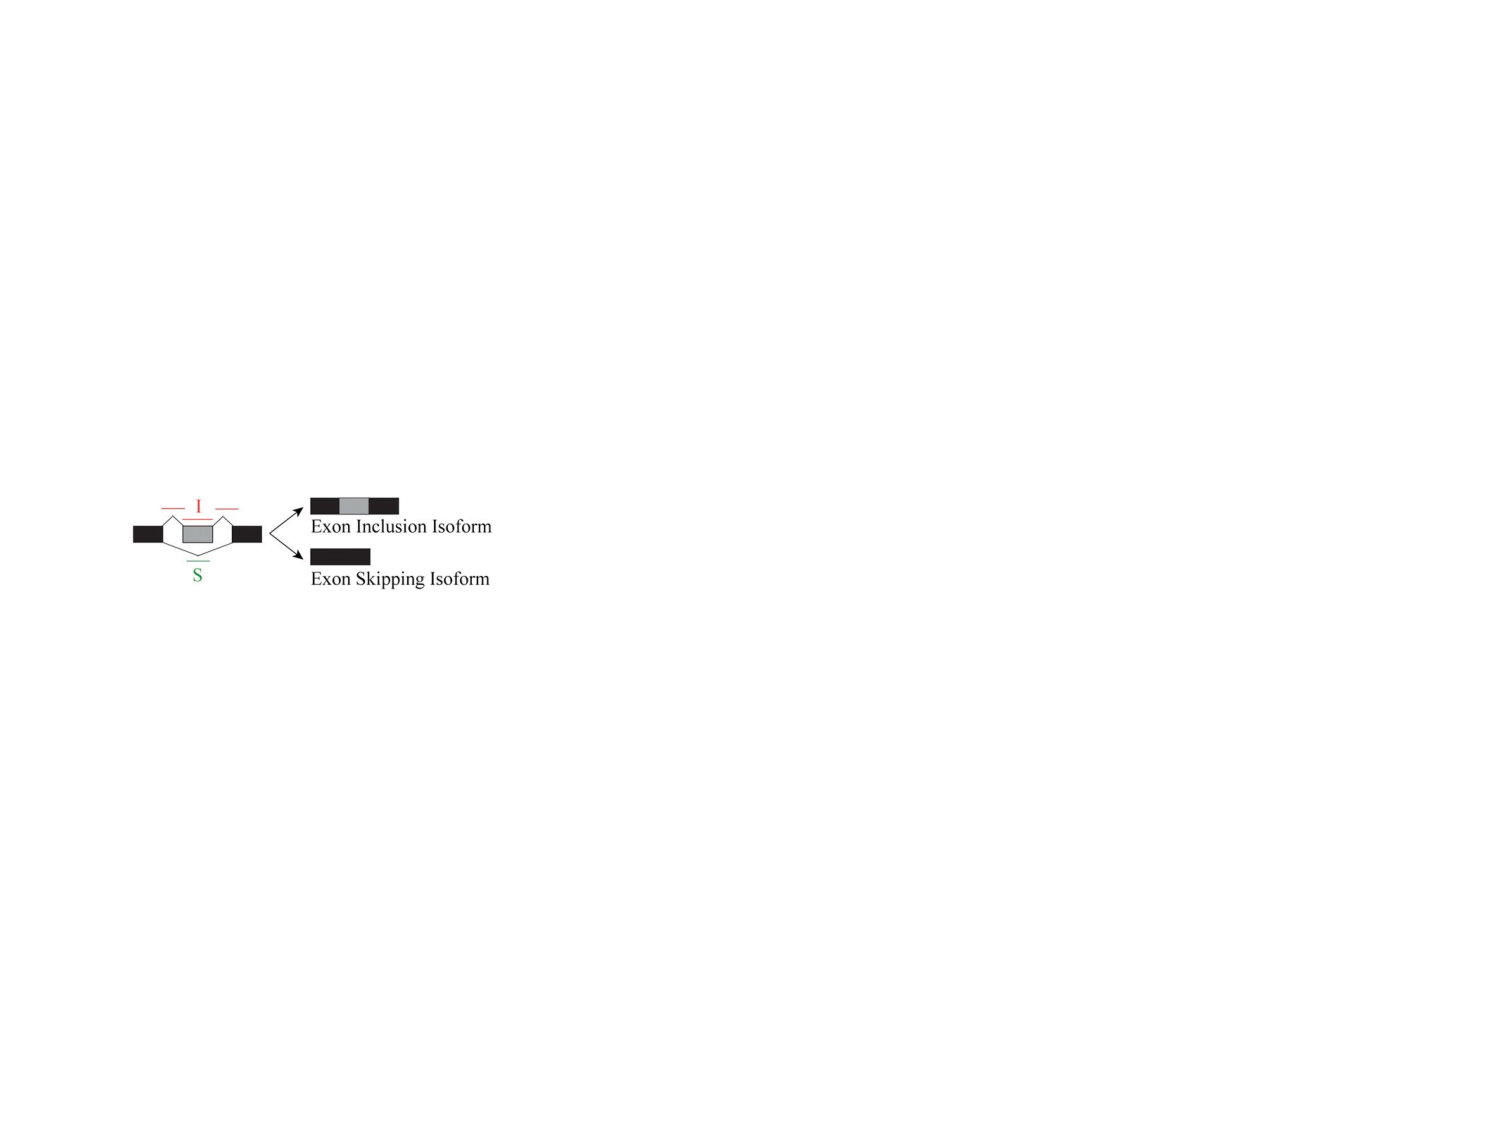
\includegraphics[width=0.7\textwidth]{img/cassette-exon.pdf}
\end{center}

\sld{Differential expression}
\begin{itemize}
\item \myemph{Multiple genes} (5000+ differentially splice in humans)
\item \myemph{Multiple groups} of cells
\begin{subitemize}
\item e.g., normal liver vs. tumor; or liver vs. kidney
\end{subitemize}
\item \myemph{Multiple subjects} in each group
\begin{subitemize}
\item i.e., biological \myemph{replicates} (cells or individuals)
\end{subitemize}
\item \myemph{Goal} is to estimate
\begin{subitemize}
\item \myemph{differential expression} between groups, and
\item \myemph{variation} within and among groups.
\end{subitemize}
\end{itemize}

\sld{Hierarchical model}
\begin{itemize}
\item \myemph{exon} $i \in 1:5000$, \ \ \myemph{group} $j \in 1:2$, \ \ \myemph{replicate} $k \in 1:K$
\item \myemph{Replicate inclusion count} (observed)
\begin{subitemize}
\item $\normalsize y_{i, j, k} \sim \textrm{binomial}(N_{i,j,k}, \ \textrm{logit}^{-1}(\psi_{i, j, k}))$
\end{subitemize}
\item \myemph{Replicate inclusion log odds}
\begin{subitemize}
\item $\normalsize \psi_{i,j,k} \sim \textrm{normal}(\phi_{i,j}, \ \sigma_{i,j})$
\end{subitemize}
\item \myemph{Group inclusion log odds}
\begin{subitemize}
\item $\normalsize \nu_i \sim \textrm{normal}(0, \tau)
\qquad
\phi_{i,1} = \theta_i + \nu_i
\qquad
\phi_{i,2} = \theta_i - \nu_i$
\end{subitemize}
\item \myemph{Gene inclusion log odds}
\begin{subitemize}
\item $\normalsize \theta_i \sim \textrm{normal}(0, \gamma)$
\end{subitemize}
\end{itemize}

\sld{Sensitivity at 95\% Specificity}
\begin{subitemize}
\item
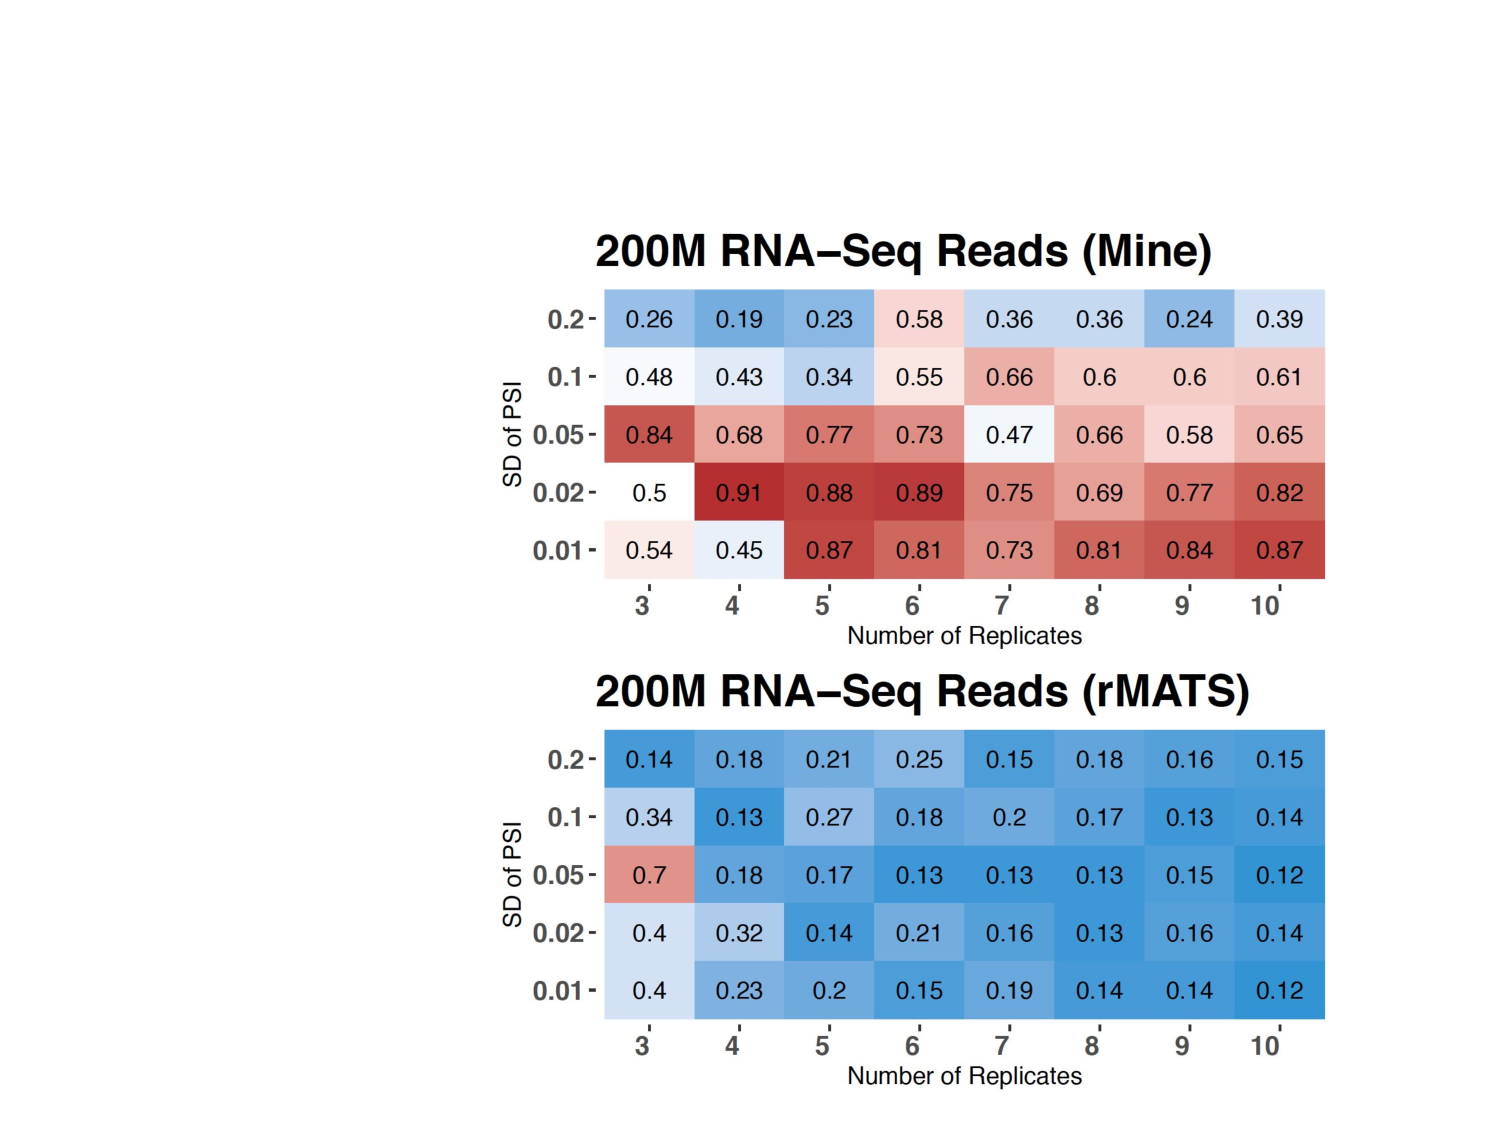
\includegraphics[width=0.50\textwidth]{img/shuonan-95pct.pdf}
\item Sensitivity = true pos.\ rate; Specificity = 1 - false pos.\ rate
\end{subitemize}

\sld{All with minimal effort}
\begin{itemize}
\item one graduate over three months part time; mostly eval
\item uses variational inference
\item Stan program for model is half a page long
\begin{subitemize}
\item hierarchical modeling automatically pools (i.e., regularizes)
\item (like jointly fitting shrinkage/regularization in ML)
\end{subitemize}
\item Eliminates pages of laborious, error-prone approximation
\begin{subitemize}
\item custom max marginal likelihood (Laplace approximation)
\item null hypothesis significance testing (likelihood ratios)
\end{subitemize}
\item 7m compute time (rMATS) vs. 10m compute time (Stan)
\end{itemize}


\mypart{}{Stan}

\sld{What is Stan?}
%
\begin{itemize}
\item a domain-specific \myemph{probabilistic programming language}
\item Stan \myemph{program} defines a \myemph{differentiable} probability model
  \begin{subitemize}
  \item declares data and (constrained) parameter variables
  \item defines log posterior (or penalized likelihood)
  \item defines predictive quantities
  \end{subitemize}
\item Stan \myemph{inference} fits model \& makes predictions
  \begin{subitemize}
  \item MCMC for full Bayesian inference
  \item variational and Laplace for approximate Bayes
  \end{subitemize}
\item \footnotesize Carpenter, B., Gelman, A., Hoffman, M. D., Lee, D., Goodrich, B., Betancourt, M., Marcus Brubaker, Jiqiang Guo, Peter Li, Riddell, A. (2017). Stan: A probabilistic programming language. {\slshape J.\ Stat.\ Soft.} 76(1).
\end{itemize}



\sld{Availability \& Usage}
\begin{subitemize}
\item \textit{Platforms:} \ Linux, Mac OS X, Windows
\vspace*{-4pt}
\item \textit{Interfaces:} \ R, Python, Julia, MATLAB, Mathematica
\vspace*{-4pt}
\item \textit{Developers (academia \& industry):} 40+ \ {\small (15+ FTEs)}
\vspace*{-4pt}
\item \textit{Users:}\ tens or hundreds of thousands
\vspace*{-4pt}
\item \textit{Companies using:} \ hundreds or thousands
\vspace*{-4pt}
\item \textit{Downloads:}\ millions
\vspace*{-4pt}
\item \textit{User's Group:} \ 3000+ registered; 6000+ non-bot views/day
\vspace*{-4pt}
\item \textit{Books using:} \ 10+
\vspace*{-4pt}
\item \textit{Courses using:} \ 100+
\vspace*{-4pt}
\item \textit{Case studies about:} 100+
\vspace*{-4pt}
\item \textit{Articles using:} \ 3000+
\vspace*{-4pt}
\item \textit{Conferences:} 4 (800+ attendance)
\end{subitemize}

\sld{Some published applications}
%
\begin{subitemize}
\item \myemph{Physical sciences}: {\footnotesize
astrophysics, statistical mechanics, particle physics, (organic) chemistry, geology, oceanography, climatology, biogeochemistry, materials science, $\ldots$
}
\vspace*{-3pt}
\item \myemph{Biological sciences}: {\footnotesize
molecular biology, clinical drug trials, entomology, pharmacology,
toxicology, opthalmology, neurology, genomics, agriculture, botany, fisheries,
epidemiology, population ecology, neurology, psychiatry, $\ldots$
}
\vspace*{-3pt}
\item \myemph{Social sciences}: {\footnotesize
 econometrics (macro and micro), population dynamics, cognitive
 science, psycholinguistics, social networks, political science,
 survey sampling, anthropology, sociology, social work, $\ldots$
}
\vspace*{-3pt}
\item \myemph{Other}: {\footnotesize education, public health, A/B testing,
government, finance, machine learning, logistics, electrical engineering,  transportation, actuarial science, sports, advertising, marketing, $\ldots$}
\end{subitemize}

\sld{Industries using Stan}
\begin{subitemize}
\item \myemph{marketing attribution}: Google, Domino's Pizza, Legendary Ent.
\item \myemph{demand forecasting}: Facebook, Salesforce
\item \myemph{financial modeling}: Two Sigma, Point72
\item \myemph{pharmacology \& CTs}: Novartis, Pfizer, Astra Zeneca
\item \myemph{(e-)sports analytics}: Tampa Bay Rays, NBA, Sony Playstation
\item \myemph{survey sampling} at YouGov, Catalist
\item \myemph{agronomy} at Climate Corp., CiBO Analytics
\item \myemph{real estate pricing models}: Reaktor
\item \myemph{industrial process control}: Fero Labs
\end{subitemize}


\sld{Why is Stan so Popular?}
\begin{subitemize}
\item \myemph{Community}: large, friendly, helpful, and sharing
\item \myemph{Documentation}:  novice to expert; breadth of fields
\item \myemph{Robustness}:  industrial-strength code; user diagnostics
\item \myemph{Flexibility}:  highly expressive language;  large math lib
\item \myemph{Portability}: popular OS, language, and cloud support
\item \myemph{Extensibility}: developer friendly; derived packages
\item \myemph{Speed}:  $2-\infty$ orders of magnitude faster
\item \myemph{Scalability}:  2+ orders of magnitude more scalable
\item \myemph{Openness}: permissive code and doc licensing
\end{subitemize}


\mypart{}{What Stan Does}

\sld{No-U-turn sampler}
%
\begin{itemize}
\item \myemph{Hamiltonian Monte Carlo} (HMC)
\begin{subitemize}
\item \myemph{Potential Energy}: negative log posterior $-\log p(\theta \mid y)$
\item \myemph{Kinetic Energy}: random standard normal each iteration
\end{subitemize}
  %
\item Adapt leapfrog algorithm \myemph{during warmup}
  \vspace*{-4pt}
  \begin{itemize}\small
  \item step size adapted to target acceptance rate
  \item Euclidean metric estimated w.\ sample covariance
  \end{itemize}
  %
\item Adapt leapfrog algorithm  \myemph{during sampling}
  \begin{subitemize}
  \item simulate forward and backward in time until U-turn
  \item multinomial sample trajectory propto energy; bias furthest
  \end{subitemize}
  %
\vfill
\hfill
{\footnotesize (Hoffman and Gelman 2011, 2014; Betancourt 2019)}
\end{itemize}

\sld{NUTS vs.\ Gibbs and Metropolis}
%
\begin{center}
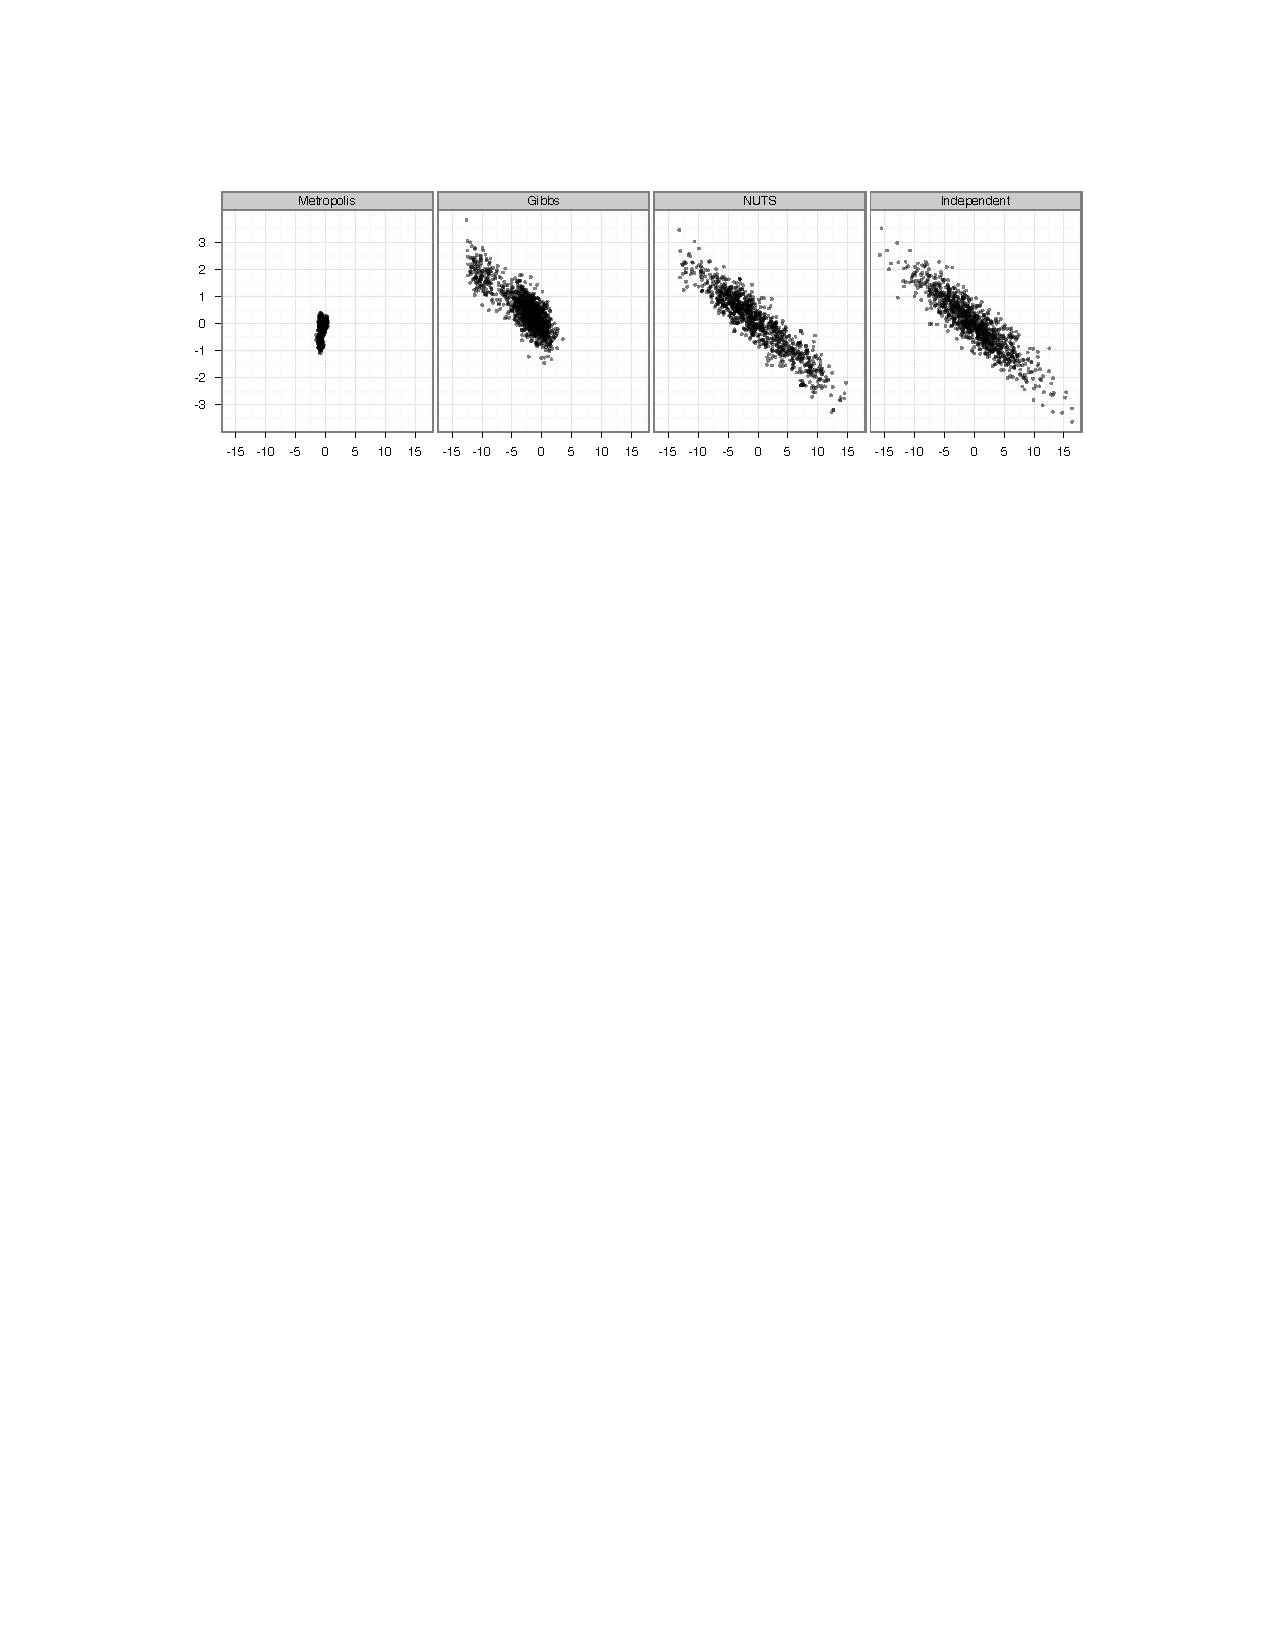
\includegraphics[width=0.9\textwidth]{img/nuts-vs.pdf}
\end{center}
\begin{subitemize}
\item Two dimensions from highly correlated 250-dim normal
\item \myemph{1,000,000 draws} from Metropolis and Gibbs (thinned to 1000)
\item \myemph{1000 draws} from NUTS; 1000 independent draws
\end{subitemize}

\sld{Reverse-mode autodiff (adjoint)}
\begin{itemize}
\item Build up expression graph with values $x$ and adjoints $\overline{x}$
\item Differentiating $f:\mathbb{R}^N \rightarrow \mathbb{R}$ is additional $\mathcal{O}(1)$
\item Set final result $y$'s adjoint $\overline{y} = 1$ and proceed in reverse
\item Example:  scalar $c = \log a$
\begin{subitemize}
\item $\overline{a} \ {+}{=} \ \overline{c} \cdot \frac{\displaystyle 1}{\displaystyle a}$
\end{subitemize}
\item Example: scalar $c = a \cdot b$
\begin{subitemize}
\item $\overline{a} \ {+}{=} \ \overline{c} \cdot b$; \ \ \ \ \
$\overline{b} \ {+}{=} \ \overline{c} \cdot a$
\end{subitemize}
\item Example: matrix $C = A^{-1}$
\begin{subitemize}
\item $\overline{A} \ {+}{=} \ -C^{\top} \cdot \overline{C} \cdot C^{\top}$
\end{subitemize}
\end{itemize}

\sld{Stan's Autodiff vs.\ Alternatives}
%
\vspace*{-4pt}
\begin{itemize}
\item Stan is \myemph{fastest} (and uses least memory)
\begin{subitemize}
\item among open-source C++ alternatives
\end{subitemize}
\end{itemize}
\vspace*{-8pt}
\mbox{ } \hfill \hfill
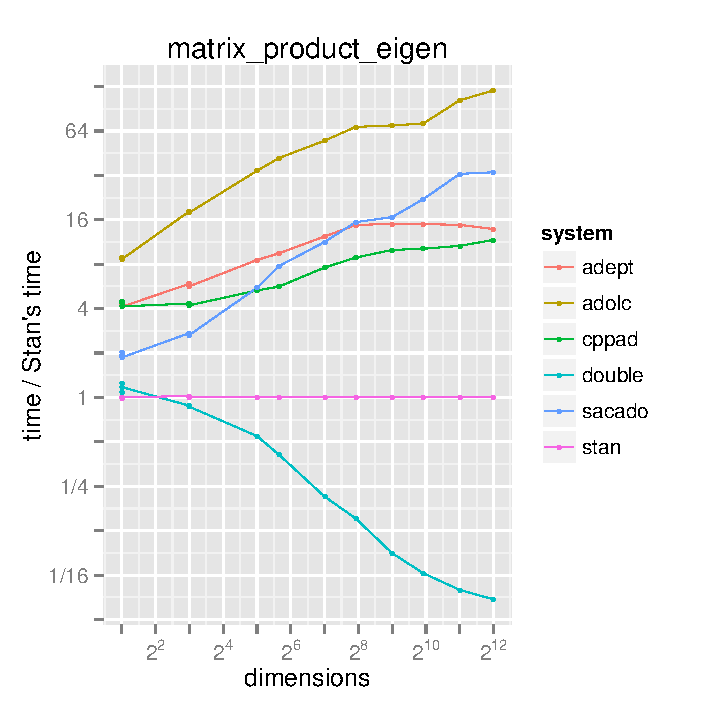
\includegraphics[width=0.40\textwidth]{img/autodiff-eval-matrix-product-eigen.pdf}
\hfill
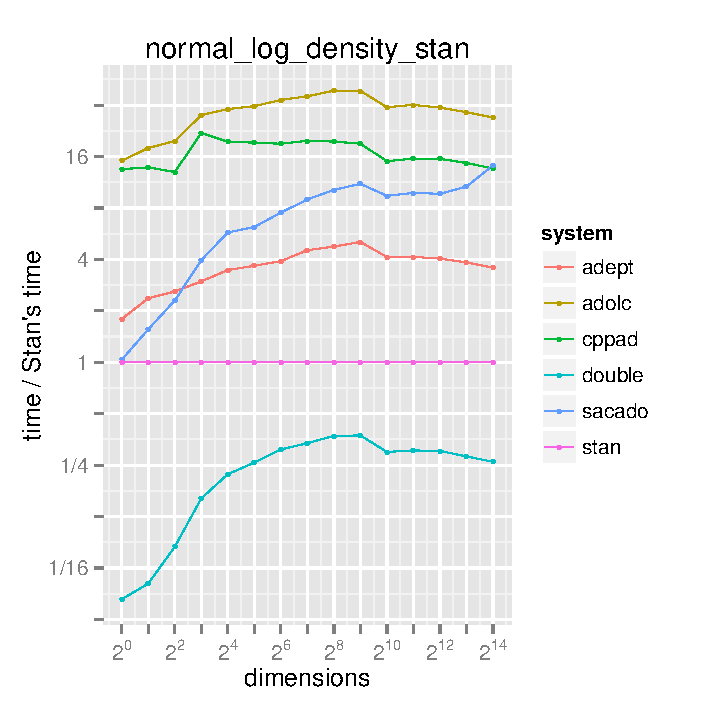
\includegraphics[width=0.40\textwidth]{img/autodiff-eval-normal-density.pdf}
\hfill \hfill
\vfill
\begin{subitemize}
\item \footnotesize Carpenter, B. et al. (2015). The Stan math library: Reverse-mode automatic differentiation in C++. {\slshape arXiv:}1509.07164
\end{subitemize}

\sld{Forward-mode autodiff (tangent)}
\begin{itemize}
\item Build tangents forward with values $x$ and tangents $\dot{x}$
\item Differentiating $f:\mathbb{R} \rightarrow \mathbb{R}^M$ is additional $\mathcal{O}(1)$
\item To differentiate w.r.t.\ $x$, set $\dot{x} = 1$ and work forward
\item Example:  scalar $c = \log a$
\begin{subitemize}
\item $\dot{c} = \dot{a} \cdot \frac{\displaystyle 1}{\displaystyle a}$
\end{subitemize}
\item Example: scalar $c = a \cdot b$
\begin{subitemize}
\item $\dot{c} = \dot{a} \cdot b + \dot{b} \cdot a$
\end{subitemize}
\item Example: matrix $C = A^{-1}$
\begin{subitemize}
\item $\dot{C} = -C \cdot \dot{A} \cdot C$
\end{subitemize}
\end{itemize}

\sld{Higher-order autodiff}
\begin{itemize}
\item Open up new algorithms exploiting curvature
\begin{subitemize}
\footnotesize
\item Riemannian HMC, nested Laplace approximations (ala INLA),
nested Jacobians for ODE solver, Newton solvers for optimizers and nested algebraic equations
\end{subitemize}
\item Considering log densities $f :\mathbb{R}^N \rightarrow \mathbb{R}$
\item Second-order derivatives
\begin{subitemize}
\item nest reverse in forward adds $\mathcal{O}(N)$
\item nest forward in forward $\mathcal{O}(N^2)$
\end{subitemize}
\item Third-order derivatives
\begin{subitemize}
\item nest reverse in forward in forward $\mathcal{O}(N^2)$
\item nest forward in forward in forward $\mathcal{O}(N^3)$
\end{subitemize}
\end{itemize}

\sld{Discrete parameters?}
\begin{itemize}
\item \myemph{Stan's focus}: tractably \myemph{marginalized}
\begin{subitemize}
\item e.g., mixtures, HMMs, state-space models
\item \myemph{efficient} in theory due to Rao-Blackwell; in practice by eliminating combinatorics; much better tail behavior
\item marginalizations available wherever you find EM \& MML
\end{subitemize}
\item \myemph{Out of scope}: combinatorially \myemph{intractable}
\begin{subitemize}
\item e.g., selection, clustering, random trees, neural nets
\item optimization is NP-hard or worse
\item thus \myemph{nobody knows how to get right} answer in general
\item some special cases can be fit
\end{subitemize}
\item \myemph{In between}: missing count data
\end{itemize}

\sld{Problems with Stan?}
\begin{itemize}
\item Failures
\begin{subitemize}
\item extreme varying posterior curvature (can't adapt)
\item stiff Hamiltonians (can't adapt)
\item floating point (e.g., log cdfs and ccdfs, gradients)
\item scalability of data and parameters
\end{subitemize}
\item Missing features
\begin{subitemize}
\item black-box log densities (cf. emcee in Python)
\item checkpointd autodiff for large Gaussian processes
\item filtering (online model updating)
\item stochastic algebraic \& diff eqs, PDEs
\item structured data types, sparse data types \& closures
\end{subitemize}
\end{itemize}

\mypart{}{Ongoing Projects}

\sld{Stan language}
\begin{itemize}
\item Extensions
\begin{subitemize}
\item lambdas with closure by value, ragged arrays, sparse matrices, tuples \& structures, user-defined gradients
\item designs: \url{https://github.com/stan-dev/design-docs}
\end{subitemize}
\item Blockless language w.\ type inference (w.\ Maria Gorinova, Sean Talts, Matthijs V\'ak\'ar)
\item Formal specification and denotational semantics (w.\ Matthijs V\'ak\'ar)
\item stanc3 parser in OCaml
\item {\footnotesize \url{https://github.com/stan-dev/stanc3}}
\end{itemize}

\sld{Blockless Stan}
\begin{itemize}
\item infers block: data, transformed data, parameter, transformed data, generated quantity
\item follows generative story
\item locates variable declarations near use
\end{itemize}
\begin{stancode}
real<lower = 0> sigma ~ lognormal(0, 1);
int K;
vector[K] beta ~ normal(0, 2);
int N;
matrix[N, K] x;
vector[N] y ~ normal(x * beta, sigma);
\end{stancode}

\sld{Algorithms}
\begin{itemize}
\item Asynchronous parallel adapation of MCMC
\item Sequential HMC for filtering (i.e., online learning)
\item Matrix automatic differentiation
\item Parallel automatic differentiation
\begin{subitemize}
\item GPU, multi-core, and multi-machine
\end{subitemize}
\item Higher-order automatic differentiation
\item prototype in R/Python; deploy in C++
\end{itemize}

\sld{Goldilocks Adaptation}
\begin{center}
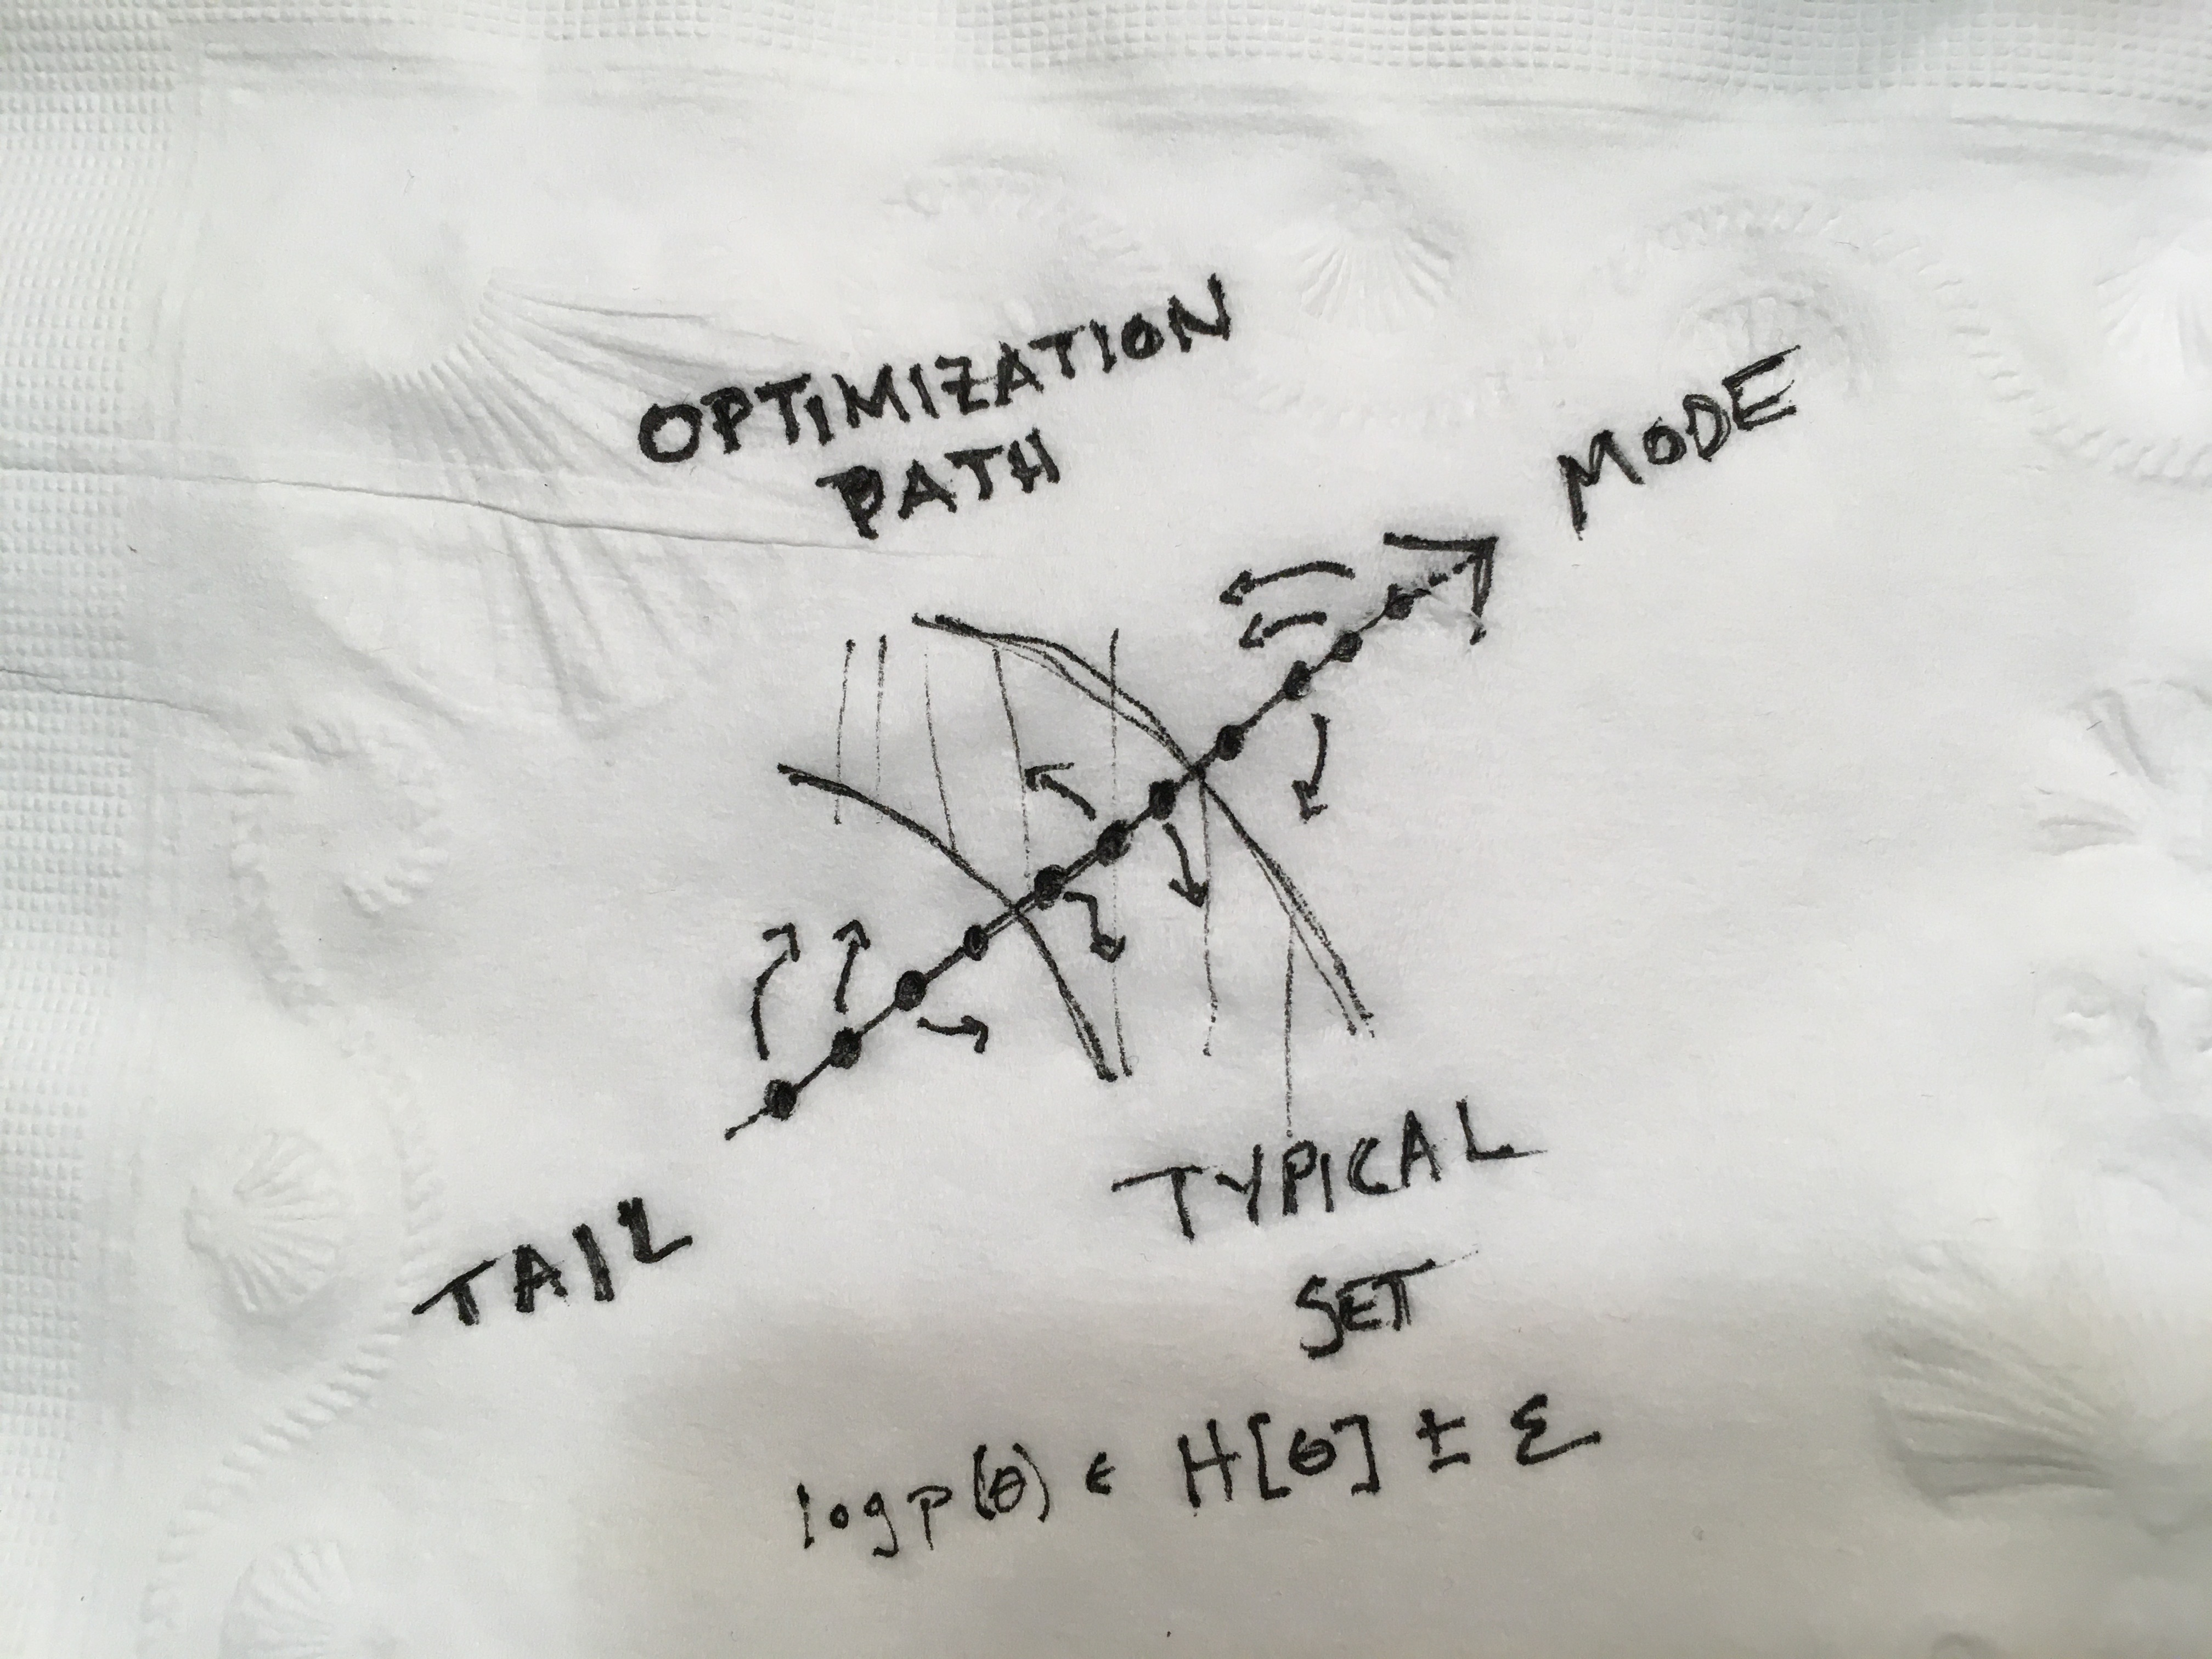
\includegraphics[width=0.3\textwidth]{img/napkin-adapt.jpg}
\end{center}
\begin{itemize}
\item Random initialize in tail; follow optimization to(ward) mode
\item At steps, spawn off depth-limited, small $\epsilon$, NUTS process
\begin{subitemize}
\item (too cold) points in tail increase log density
\item (too hot) points toward mode decrease in log density
\item (just right) those in typical set follow flow inside
\end{subitemize}
\end{itemize}

\sld{Methodology}
\begin{itemize}
\item Bayes vs.\ point estimation \& proper scoring
\item Model/data evaluation via calibration and sharpenss (entropy)
\item Model/data evaluation with uncertain (crowdsourced) data
\item Partially pool performance estimates for multiple comparison
\item Push uncertainty through decision making
\vfill
\noindent
{\footnotesize Work in progress: \url{https://github.com/bob-carpenter/case-studies}}
\end{itemize}

\sld{Arctic soil-carbon response}
\begin{itemize}
\item collect low arctic aquatic to high arctic terrestrial soil carbon data over time
\item soil carbon dynamics models with biochemical components and environment covariates
\item Kathe Todd-Brown (U.\ Florida, environmental engineering)
\item Sean Schaeffer (U.\ Tennessee, agriculture)
\vfill
\item {\footnotesize NSF proposal under review (PI)}
\end{itemize}

\sld{Differential expression of isoforms}
\begin{itemize}
\item hierarhcical modeling for group and individual and cellular variation
\item inferring splice variants in cassette exons and more generally
\item Shuonan Chen (Columbia, biostatistics)
\item Chaolin Zhang (Columbia, genomics)
\vfill
\item \footnotesize{Shuonan writing up for submission and open-source release}
\end{itemize}

\sld{Virtual database for elections}
\begin{itemize}
\item for Cooperative Congressional Election Study
\item scaling/applying multilevel regression and poststratification
\item visualization and deployment of virtual database
\item survey statistics
\item Steve Ansolabehere (Harvard, political science))
\item Andrew Gelman (Columbia, stats)
\item Ben Bales (Columbia, Earth Institute)
\vfill
\item {\footnotesize \$900K NSF grant recently awarded (co-PI)}
\end{itemize}

\sld{Ed.\ testing and hier.\ modeling}
\begin{itemize}
\item improved multilevel model fitting
\item applications in education with nested students/teachers
\item Sophia Rabe-Hesketh (UC Berkeley, education \& biostatistics)
\item Andrew Gelman (Columbia, stats)
\item Ben Goodrich (Columbia, ISERP)
\vfill
\item {\footnotesize \$400K IES grant recently awarded (co-PI)}
\item {\footnotesize previous IES grant: \url{https://education-stan.github.io}}
\end{itemize}

\sld{Auction pricing and equilibrium}
\begin{itemize}
\item equilibrium \& rational decision making in auction pricing
\item improved differential and algebraic equation solving
\item Tom Sargent (NYU, economics)
\item Shoshanna Vasserman (Stanford, business)
\item Andrew Gelman (Columbia, stats)
\vfill
\item {\footnotesize \$350K Alfred P. Sloan Foundation grant awarded (co-PI)}
\end{itemize}

\sld{Pharmacokinetics and disease}
\begin{itemize}
\item pharmacokinetics and dynamics for disease modeling
\item adding partial differential equations
\item adding differential algebraic equations
\item evaluating variational inference
\item Yi Zhang (Metrum, LLC, applied math)
\item Bill Gillespie (Metrum, LLC, pharmacology)
\item Andrew Gelman (Columbia, stats)
\vfill
\item {\footnotesize \$900K ONR Phase II STTR grant awarded (co-PI)}
\end{itemize}

\sld{Crowdsourced machine learning}
\begin{itemize}
\item apply crowdsourced data to learning
\item apply crowdsource data to evaluation
\item Bayesian models of data annotation/coding
\item Massimo Poesio (U. Essex, computer science)
\item Silviu Paun (U. Essex, computer science)
\item Becky Passonneau (Penn State, computer science)
\vfill
\item \footnotesize \url{https://transacl.org/ojs/index.php/tacl/article/view/1430}
\item \footnotesize \url{https://transacl.org/ojs/index.php/tacl/article/view/389}
\end{itemize}

\sld{Book}
\begin{itemize}
\item I'm halfway done with a second book:
\begin{quote}
Carpenter, Bob. (forthcoming) \myemph{\slshape Probability and Statistics: A Simulation-Based Introduction.}
\end{quote}
\begin{subitemize}
\item for \myemph{upper-level undergrad/grad} students in sciences, etc.
\item goal is to bring up to speed with \myemph{statistical computation}
\item fully \myemph{reproducible}, open-source
\item assumes limited facitlity with \myemph{calculus \& linear algebra}
\end{subitemize}
\vfill
\noindent
{\footnotesize Draft: \url{https://github.com/bob-carpenter/prob-stats}}
\end{itemize}

\sld{Summary: List of Projects}
\begin{subitemize}
\item \myemph{Stan language} (structs; closures; sparse; ragged; blockless)
\item \myemph{applied math algorithms} (autodiff; numerics)
\item \myemph{MCMC algorithms} (adaptation; sampling; sequential)
\item \myemph{Applications}
\begin{subitemize}
\item arctic soil carb; differential isoform expression; virtual election DB;
educational testing; auction pricing and equilibrium; pharmacokinetics and
disease modeling; crowdsourced machine learning
\end{subitemize}
\item \myemph{book} on probability \& stats via simulation
\end{subitemize}



\mypart{}{Canned Answers}

\sld{TensorFlow or PyTorch?}
\begin{itemize}
\item embedded in Python
\item similar scope to Stan's differentiable math library
\item TensorFlow optimizes static autodiff; Pytorch dynamic (like Stan)
\item focused on approximate optimization algorithms
\item optimized for neural networks on distributed architecture
\end{itemize}

\sld{TensorFlow Probability?}
\begin{itemize}
\item embedded in Python
\item similar performance to Stan
\item adds stats functions to TensorFlow
\begin{subitemize}
\item catching up to Stan with growing staffing
\end{subitemize}
\item adds inference algorithms on top
\begin{subitemize}
\item main focus is approximate inference \& deep neural nets
\item recently added static parallel NUTS implementation
\end{subitemize}
\item Edward(2) moribund
\end{itemize}

\sld{PyMC4?}
\begin{itemize}
\item embedded in Python
\item replacing Theano analytic diff with TensorFlow autodiff
\item supported by Google
\item more limited library and control flow than Stan
\item more flexible sampling algorithm combination (e.g., discrete)
\item borrowed Stan's HMC algorithms and diagnostics
\item {advantage} is {embedding of language} as Python API
\item {disadvantage} is {limited flexibility} (not arbitrary Python)
\end{itemize}

\sld{Pyro}
\begin{itemize}
\item embedded in Python
\item based on dynamic PyTorch, so most like Stan
\item main focus approximate inference \& deep neural nets
\item borrowed Stan's HMC algorithms and diagnostics
\end{itemize}

\sld{Roll my own sampler?}
\begin{itemize}
\item It's a tricky business, so only as a last resort
\begin{subitemize}
\item specific difficulties arise from non-determinism,
floating point, and failures of geometric ergodicity
\end{subitemize}
\item Sometimes it's the only option
\begin{subitemize}
\item known scalable algorithms require derivatives at first-order or higher
\item carefully validate with simulation-based calibration
\item when it works, let us know, and we can put it in Stan!
\end{subitemize}
\end{itemize}


\end{document}
